%%%%%%%%%%%%%%%%%%%%%%%%%%%%%%%%%%%%%%%%
% Chapter 2: What is synthetic data
%%%%%%%%%%%%%%%%%%%%%%%%%%%%%%%%%%%%%%%%


\label{syntheticdata}

In short, synthetic data is artificially manufactured data. Synthetic data can encompass a wide range of data types, mirroring the diversity found in real-world datasets. It can be used for both structured data, such as tabular data where rows represent individual records and columns represent attributes, and unstructured data such as text, images, and audio. Examples of synthetic tabular data are health records, customer information, transaction records, and clinical trial data \cite{el2020practical,yan2022multifaceted,hradec2022multipurpose}. Unstructured synthetic data includes chat logs, emails, social media posts and clinical notes for text \cite{sagduyu2018synthetic,li2021synthetic}, and medical scans and deepfakes for images \cite{patel2023deepfake,paproki2024synthetic}. 

Two main types of synthetic data can be differentiated: synthetic data that is created from scratch and not based on a particular real-world dataset, and synthetic data that is generated to mimic a (complete or partial) real-world dataset. 

\section{Creating synthetic data from scratch}
Synthetic data generated from scratch is entirely artificial and created without using any real-world data as a template. This type of synthetic data is constructed using mathematical models and algorithms that define specific characteristics of the data. For instance, researchers can use simulation techniques to generate datasets based on theoretical distributions and hypothetical scenarios, or their own domain-specific knowledge. This approach is particularly useful for testing hypotheses, developing algorithms, and conducting simulations where real-world data is either unavailable or unsuitable. Because it is not derived from actual data, synthetic data from scratch poses very little risk of compromising privacy \cite{el2020practical,soltana2017synthetic}. 

\vspace{5pt}
\begin{figure}[h!]
    \centering
    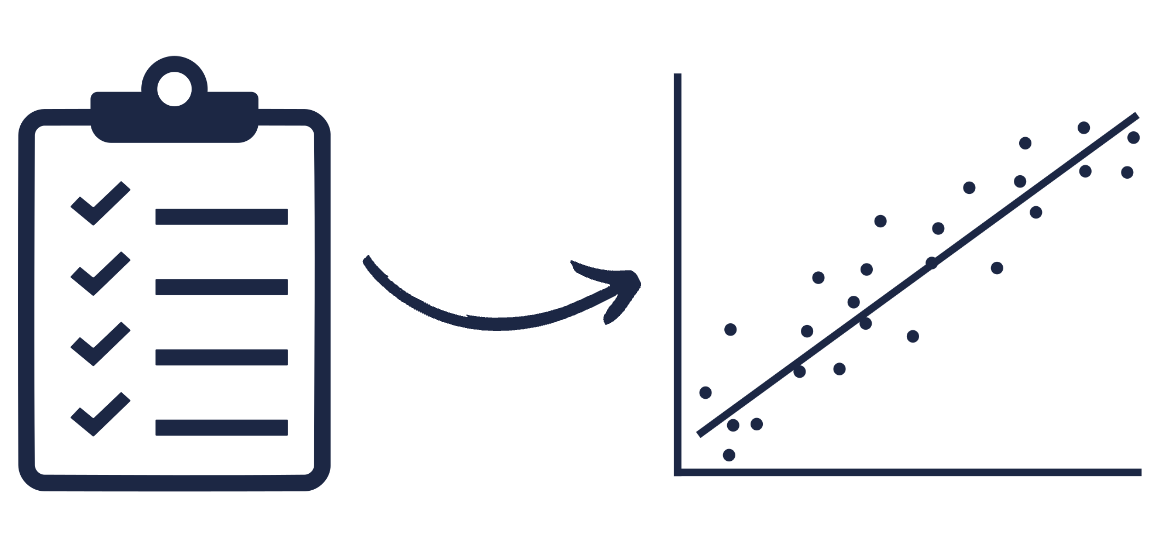
\includegraphics[width=0.5\textwidth]{Images/SyntheticData_1.png}
    \caption{Synthetic data from scratch.}
    \label{fig:sample_image}
\end{figure}
\vspace{5pt}

\section{Creating synthetic data based on real-world data}
Synthetic data designed to mimic-real-world data, on the other hand, is generated using real datasets as a basis. Advanced algorithms, including machine learning and deep learning techniques, are employed to analyse the patterns and relationships within the real data. These patterns are then used to generate synthetic data that closely mirrors the statistical properties and structure of the original dataset. The goal is to produce synthetic data that is realistic enough to be used in place of actual data for analysis, testing, training, or informative purposes while ensuring that no individual's personal information is exposed. This type of synthetic data is particularly valuable in fields like healthcare, finance, criminology or other social sciences, where data privacy is paramount but the need for realistic data is critical for effective research and development \cite{arnold2020really, jordon2022synthetic}. \\

\vspace{10pt}
\begin{figure}[H]
    \centering
    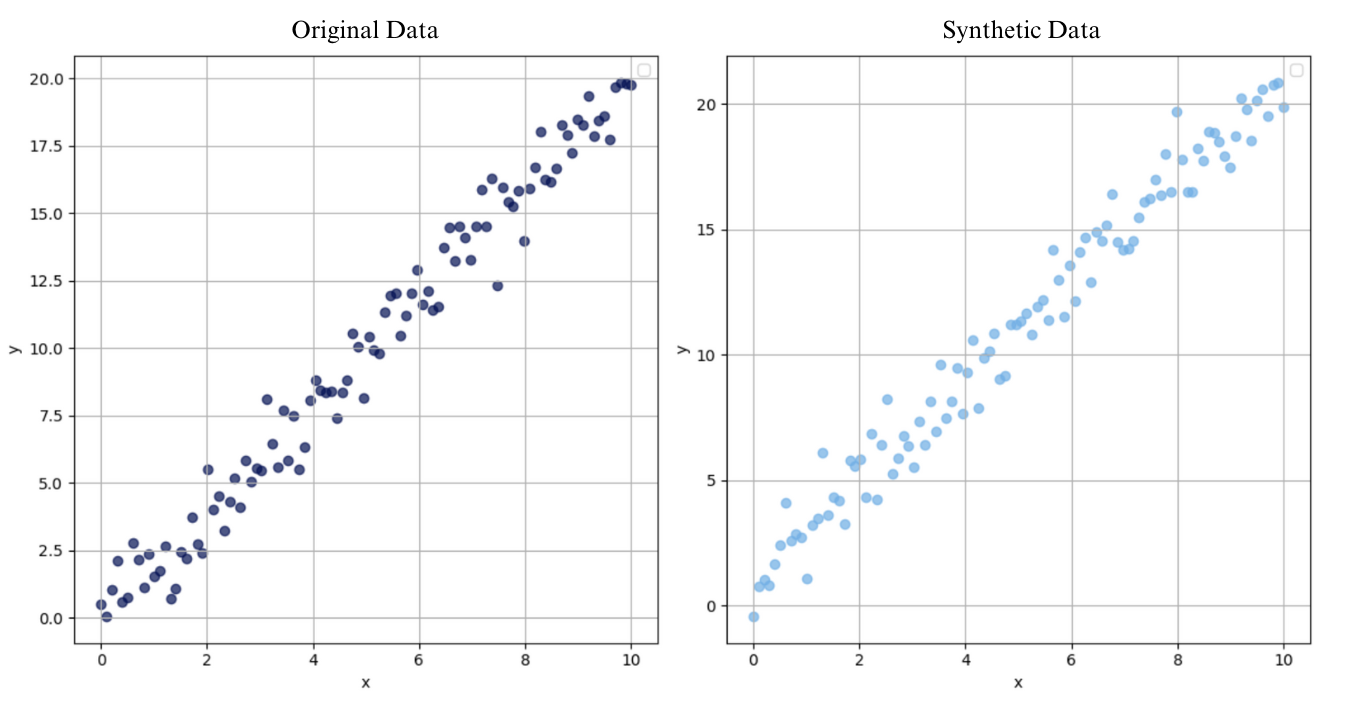
\includegraphics[width=\textwidth]{Images/Screenshot 2024-08-06 at 12.32.53.png}
    \caption{Synthetic data mimicking real-world data.}
    \label{fig:synthesis_2}
\end{figure} 
\vspace{10pt}


By understanding and utilising these two types of synthetic data, researchers can overcome many of the challenges associated with data privacy and sharing. Synthetic data from scratch provides a risk-free environment for preliminary research and hypothesis testing, while synthetic data that mimics real-world data enable researchers to perform realistic and meaningful analyses without compromising the privacy of individuals. Together, these approaches offer solutions for enhancing data sharing and collaboration in compliance with privacy regulations. 

\section{Advantages and disadvantages of synthetic data}

Synthetic data both provides significant benefits, whilst also presenting unique challenges. This section summarises some of the main advantages and disadvantages of synthetic data. Some of these are discussed more in-depth in the following chapters.

\textbf{Benefit: Privacy preservation}\\
Synthetic data can be generated without compromising sensitive information, making it an excellent tool for privacy-preserving data analysis. This is particularly relevant for fields that work with sensitive data, such as healthcare data, financial data or crime data, where data privacy regulations like GDPR and HIPAA are stringent. By using synthetic data, organisations can share and analyse data without exposing personally identifiable information and harming someone's right to privacy. 

\textbf{Benefit: Data augmentation}\\
Synthetic data is invaluable for augmenting small datasets. In fields such as machine learning, large datasets are crucial for training robust models. Synthetic data can fill gaps, balance class distributions, and enhance the diversity of training data, leading to improved model performance.

\textbf{Benefit: Cost-effective}\\
Generating synthetic data can be more cost-effective than collecting and labelling real-world data. Data collection processes can be expensive and time-consuming, often requiring significant human resources. Synthetic data, on the other hand, can be produced at a fraction of the cost and time.

\textbf{Benefit: Data- and environment manipulation}\\
Synthetic data allows for the creation of controlled environments where variables can be manipulated to study their effects. This is beneficial in scientific research and simulation studies, where researchers can systematically vary parameters and observe outcomes without real-world constraints.  

\textbf{Disadvantage: Quality concerns}\\
The quality of synthetic data depends heavily on the models used to generate it. Poorly designed synthetic data may not accurately reflect real-world patterns and correlations, leading to misleading conclusions and poorly performing machine learning models. So far, there are no standardised frameworks for quality control of synthetic data.

\textbf{Disadvantage: Potential biases}\\
Data can include various biases, from cultural biases to technological biases. Biases in data become particularly problematic when biased (synthetic) data is used to inform policies. If the models generating synthetic data are trained on biased real-world data, these biases can be perpetuated or even enhanced in the synthetic data. This can lead to biased outcomes in analyses and machine learning models, undermining the benefits of using synthetic data. Thus, biases need to be identified in real-world data and mitigated in the process of data synthesis when necessary \cite{barbierato2022methodology}.

\textbf{Disadvantage: Complexity of data generation}\\
Generating high-quality synthetic data can require advanced knowledge in data science, statistics, and domain-specific expertise for the evaluation of synthetic data. Developing and fine-tuning the synthesis process and associated models can be complex and time-consuming, requiring specialised skills and computational resources. Moreover, in many fields, there are no good examples yet of the generation and application of synthetic data.

\textbf{Disadvantage: Regulatory and ethical concerns}\\
While synthetic data can help navigate privacy regulations, it is not free from regulatory scrutiny. Misuse of synthetic data, especially when it comes to mimicking sensitive data, can raise ethical and legal issues. Furthermore, reliance on synthetic data must be carefully managed to avoid overestimating its reliability and validity, given possible quality control problems. 


\section{Potential uses for synthetic data in scientific research}

The potential of synthetic data for scientific research is plentiful, given its ability to replicate real-world data patterns while preserving privacy and circumventing data access limitations.

In \textbf{healthcare}, synthetic data plays a crucial role in medical research and clinical trials. Researchers can generate synthetic patient records that mimic real-world medical histories, allowing for the development and testing of new treatments and diagnostic tools without risking patient confidentiality. For example, synthetic data can simulate patient outcomes in clinical trials, providing a safe environment to asses the effectiveness and safety of new drugs before conducting actual trials. \cite{gonzales2023synthetic,arora2022generative,braddon2023exploring}

In \textbf{finance}, synthetic data is used to model financial markets and economic behaviour. Researchers can generate synthetic stock market data, transaction records, and costumer profiles to test trading algorithms and risk management strategies without exposing sensitive financial information. This approach not only safeguards privacy but also allows researchers to conduct extensive stress testing and scenario analysis, which is essential for understanding market dynamics and preparing for potential economic crises. \cite{assefa2020generating,eckerli2021generative}

\textbf{Environmental science} benefits from synthetic data through the simulation of environmental phenomena and the modelling of ecosystems. For instance, researchers can generate synthetic climate data to study the impacts of climate change under various scenarios. This include simulating temperature variations, precipitation patterns, and extreme weather events to predict their effects on ecosystems and human societies. Synthetic data also aids in the development of predictive models for natural disasters, such as floods and hurricanes, enhancing preparedness and response strategies. \cite{kravitz2021potential,perez2021machine}

In the fields of \textbf{criminology}, synthetic data is utilised to analyse crime patterns and develop predictive policing models. By creating synthetic crime reports and incident data, researchers can study trends and correlations without compromising the privacy of individuals involved in real criminal cases. This helps in identifying risk factors, improving law enforcement strategies, and designing more effective crime prevention programs. \cite{brunton2024using}

\textbf{Social sciences} also leverage synthetic data to study human behaviour and societal trends. Researchers can generate synthetic survey responses, demographic data, and social interactions to explore phenomena such as voting behavior, social mobility, and public opinion. This enables the examination of various hypotheses and policy impacts without the ethical and practical challenges associated with collecting real-world data. \cite{hradec2022multipurpose,kokosi2022overview}

\newpage
\subsection{The use of synthetic data for open science practices}

Next to these practical applications, synthetic data offers several compelling advantages for open science practices and the FAIR principles. 

\textbf{Privacy preservation}\\ 
One of the most significant benefits of synthetic data is its ability to preserve privacy. Open science advocates for data sharing to foster transparency and reproducibility, but sharing real-world data often conflicts with privacy concerns, especially in sensitive fields like healthcare, medicine or social sciences. Synthetic data, which mimics real data without containing personal information, allows researchers to share datasets freely without risking breaches of confidentiality.

\textbf{Data accessibility}\\ 
Synthetic data facilitates broader access to data. Researchers can generate and share synthetic datasets that replicate the properties of restricted or proprietary data. This accessibility aligns with the FAIR principle of making data accessible, enabling a wider community of researchers to engage with and analyse the data, thus promoting inclusivity and collaboration. 

\textbf{Enhanced interoperability}\\
By using standardised methods and tools to generate synthetic data, researchers can ensure that datasets are compatible across various platforms and software. This interoperability is crucial for collaborative efforts where multiple teams might be using different systems and tools, allowing for seamless integration and analysis of data from diverse sources. 

\textbf{Reusability}\\
Synthetic data enhances the reusability of datasets. Because it can be shared without legal or ethical restrictions, synthetic data can be reused in multiple studies and by various research teams. This reusability supports the FAIR principle by maximising the utility of datasets, enabling continuous testing and validation of scientific hypotheses, and facilitating cumulative knowledge building. 

\newpage
\textbf{Cost-effectiveness and efficiency}\\
Generating synthetic data can be more cost-effective and time-efficient than collecting new data. This efficiency allows researchers to quickly produce large, rich datasets necessary for robust scientific inquiry. Additionally, synthetic data can simulate rare or hypothetical scenarios, providing valuable insights that might be difficult or impossible to obtain from real-world data. \\

Overall, synthetic data significantly advances open science and the FAIR principles by enhancing privacy, accessibility, interoperability, and reusability. It empowers researchers to share and utilise data more freely and effectively, fostering a more collaborative and transparent scientific environment. 

\subsection{Synthetic data compared to other privacy-preserving methods}
The generation of synthetic data is not the first or only mechanism through which researchers can enhance and protect the privacy of their data. Other common mechanisms include anonymisation and differential privacy, yet both come with significant shortcomings.

\textbf{Anonymisation} involves removing or obfuscating personally identifiable information from dataset to prevent the identification of individuals. This method can be as easy as deleting attributes in a dataset that are related to personal information, such as names of individuals. As such, anonymisation is a widely used method. However, anonymisation has significant limitations, particularly in the face of advanced re-identification techniques. Even anonymised datasets can sometimes be linked with other data sources to re-identify individuals, compromising privacy. This limitation is especially pertinent in the era of big data, where vast amounts of auxiliary information are readily available \cite{majeed2020anonymization}. Additionally, obfuscating information which may be relevant may harm the overall utility of the dataset.

\textbf{Differential privacy} is another privacy-preserving mechanism \cite{dwork2006differential}. Differential privacy is a sophisticated technique that adds controlled noise to datasets, ensuring that the inclusion or exclusion of any single data point does not significantly affect the overall results. For example, noise can be added by altering certain values to obscure the exact, personal information. For example, amounts of salaries can be multiplied by a certain number, keeping the relative differences intact. This method provides strong mathematical guarantees of privacy and is particularly effective in preventing re-identification. However, the added noise can degrade data utility, making it less useful for certain types of analyses. Using the example of altered salaries, whilst a multiplication of the actual salary may keep the relative salary differences between employees intact, but does not allow for a comparison with the national average. Implementing differential privacy also requires careful calibration to balance privacy and data quality, which can be complex and resource-intensive \cite{wasserman2010statistical,wood2018differential}. Additionally, it should be noted that differential-privacy can also be employed \textit{within} synthetic data generation, as a means to prevent re-identification from a synthetic dataset \cite{jordon2018pate,xin2022federated,sun2023generating}. \\


Each of these privacy-preserving methods comes with its own benefits and challenges. The choice of mechanism depends on the specific requirements and constraints of the research project.